


\section{Numerical Analysis}

In order to validate the approximations made in previous sections, we solve system \ref{eq:system} numerically. In order to do so, we use the Runge-Kutta Method of order 4 along with the  Shooting Method to solve the two point boundary value (reference to Numerical Methods in python).  



The complexity of the problem lies exactly in the two point boundary feature of the problem, where the concentrations are known in the bulk, but the potential is known at the interface(see Fig. \ref{fig:geometry}). 

The approach used in these type of problems is transforming the second order system \ref{eq:system} into a first order one,

\begin{eqnarray}
C'_+(x)-\frac{zF}{RT}E(x)C_+(x) &=& -r, \\
C'_-(x)+\frac{zF}{RT}E(x)C_-(x) &=& 0, \\
E'(x) &=& \frac{zF}{\epsilon}(C_+(x)-C_-(x)), \\
\phi'(x) &=& -E(x).
\label{eq:linear-system}
\end{eqnarray}

subject to the border conditions

\begin{eqnarray}
C_+(\delta) &= C_b,  \\
C_-(\delta) &= C_b, \\
\phi(\delta) &=& 0\\
\phi(0) &=&  V_0
\label{eq:linear-system}
\end{eqnarray}

Here the primes denote derivatives with respect to $x$. Once the system is in the form of Eqn. \ref{eq:linear-system}, we can apply the Runge-Kutta Method with the shooting method to obtain the numerical solutions. 


\section{Results}

Fig. \ref{fig:numeric-results} show the results obtained. The solution of the steady state at different values of the reaction rate do not defer much closest to the surface of the electrode ($x=0$). Also, from Fig. \ref{fig:numeric-results} (c) and (d) we can see that the aproximation of the electric field and the electric potential is fairly 

\begin{figure}[htbp]
 \centering
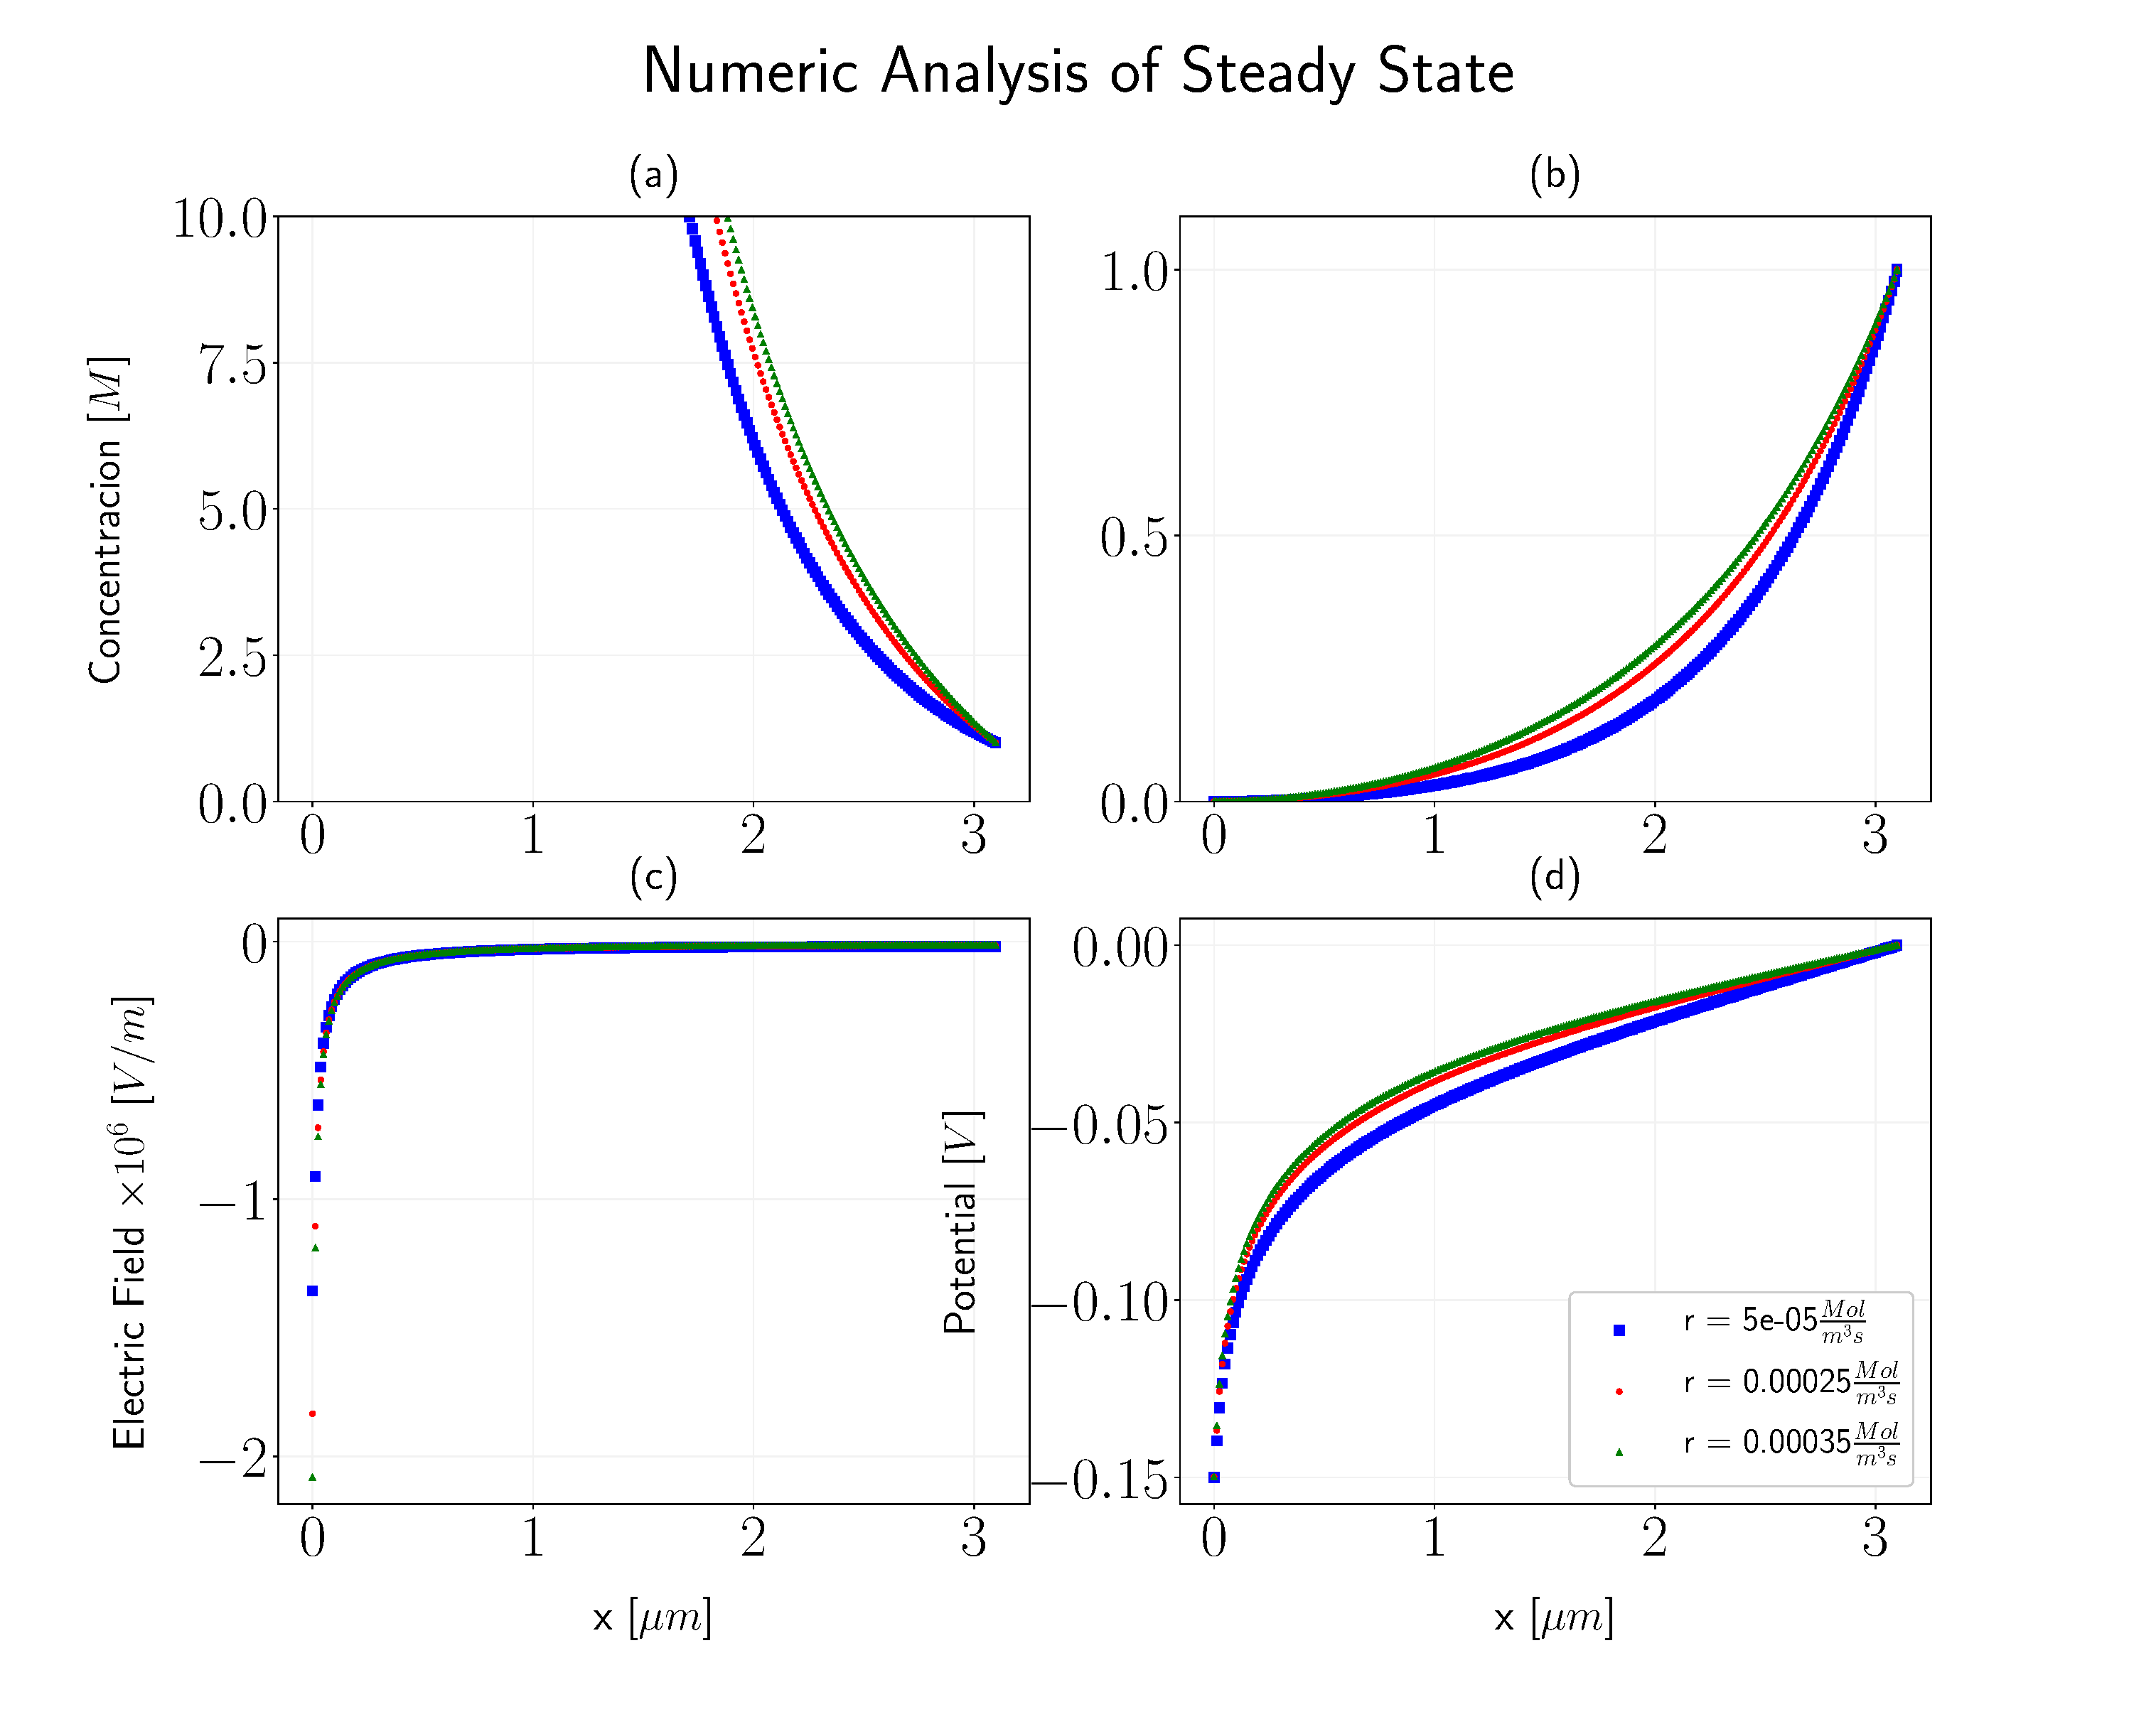
\includegraphics[width = \linewidth]{results-numeric}
 \caption{The numerical and the analytic solution to the potential to first order in the current.}
 \label{fig:numeric-results}
\end{figure}

Dealing with the equations as presented in Eq. \ref{eq:system} is extremely difficult when doing a numerical analysis. This is due to the fact that the natural units of the system (x which is measured in meters) are too small for the computer to handle. Also, non-linearity gives extreme fluctuations of the concentration of the positive ion near the surface. Since we where using the shooting method, we needed to change the values of the electric field at the bulk, such that the boundary condition for the electric potential is correct, but this induced such strong concentrations at the interface sometimes, that the computer could not handle the numbers resulting from Runge-Kutta method. We had to make a little adaptation in order to be able to find the correct boundary condition for the electric field with the shooting method. 




As it can be seen in figures  \ref{fig:numerical-phi},  \ref{fig:numerical-E}, the electric field and potential approach zero when the start moving into the bulk of the solution, as expected. The further away from the interface we go, the better the border conditions for the electric field are met. For our particular case, we cut the integration range when we reached a tolerance of $ E_{bulk} < 1\times 10^{-3}$, where $E_{bulk}$ is the border condition of the dimensionless electric field at the bulk. 



A similar analysis can be done for the concentrations (Fig.  \ref{fig:numerical_c}), but this time the value of both concentrations at the bulk is $C_b$, as defined by the border conditons for the system \ref{eq:system}.



Another difficulty is that, since we used the adaptive Runge-Kutta method, the concentrations change so abruptly that the adaptive step $h$ becomes increadibly small. The problem with this is that the number of iterations needed with a step of the order of $h\approx 10^{-29}$. In order to reach the full length of integration is too big and therefore, we obtain only a part of the integration interval and not as close to the interface as we should like. 

To avoid such difficulties, we have worked with the adimensional potential in a scale of adimensional length $\xi = \kappa x$. We have integrated on the interval $[0, 20 \kappa \delta]$.


